\begin{frame}
\section{}
Complete the following implementation of Xavier initialization where weights are initialized as $W_l = \mathcal{N}(\mu=0,\sigma^2=\frac 1 {n_{l-1}})$ where $W_l$ denotes weights of layer $l$ and $n_{l-1}$ denote number of nodes in layer $l-1$

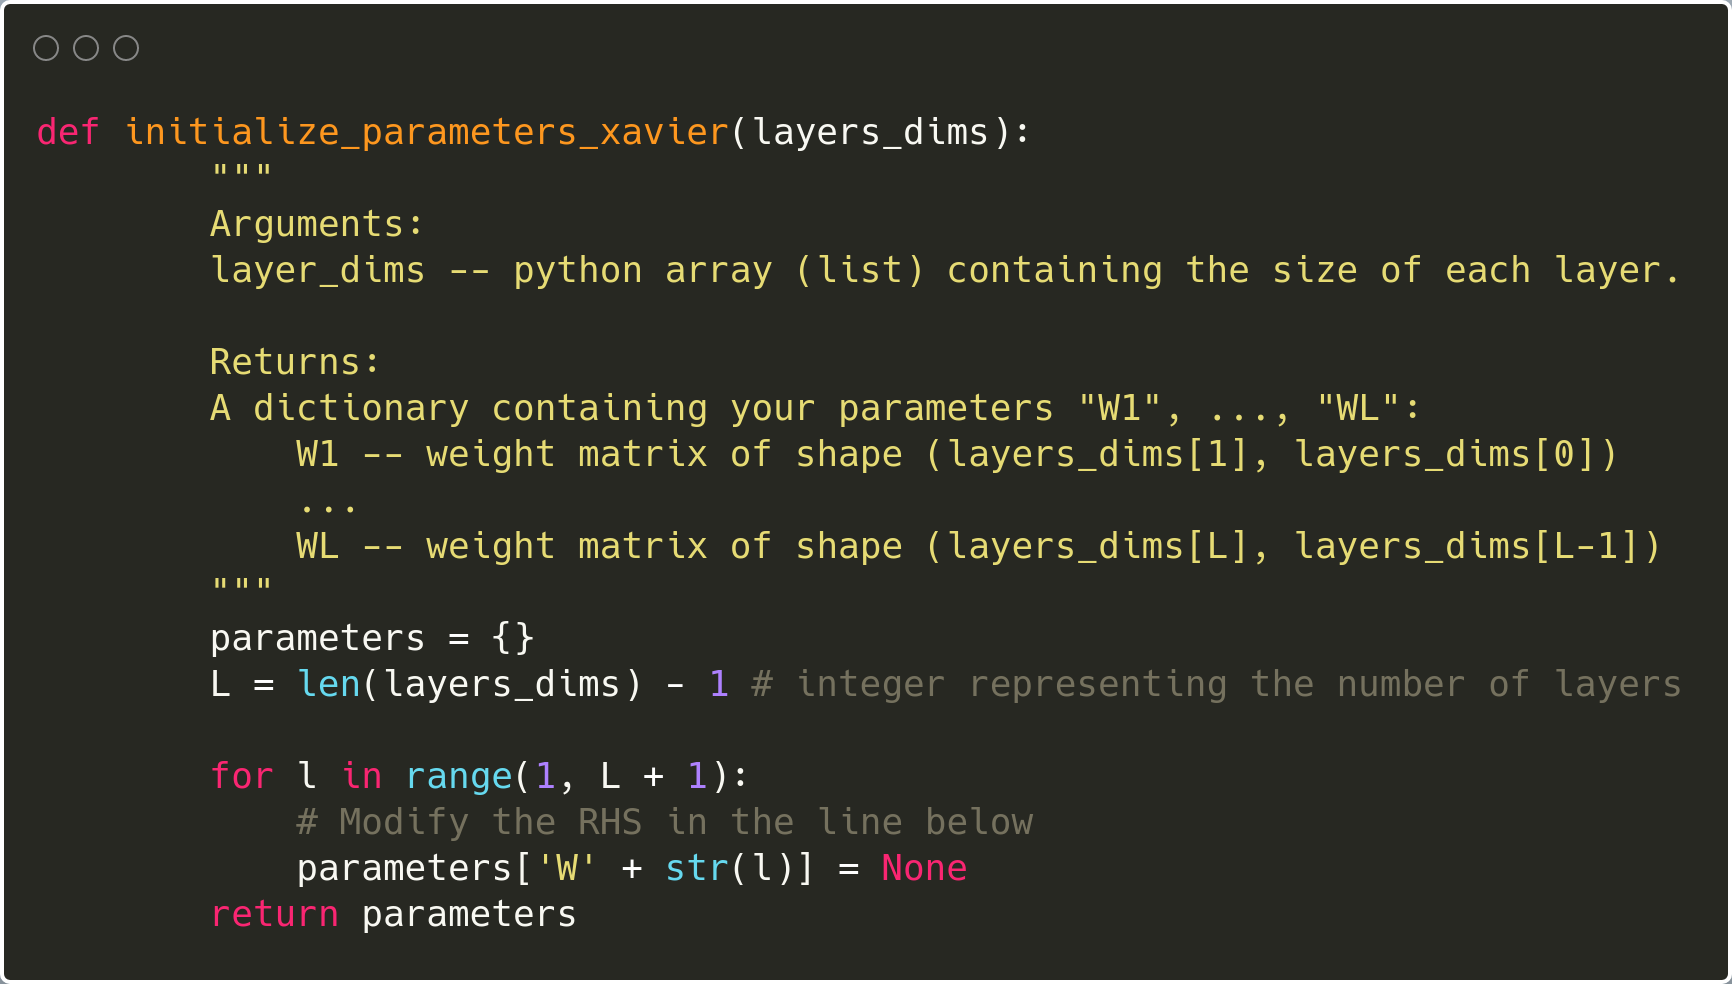
\includegraphics[width=0.8\textwidth]{images/quiz_4_4_1_1.png}

You can use either numpy or PyTorch. Please write the line of code below the comment "Modify the RHS.."


% FIB

\end{frame}

\begin{frame}
\section{}
Complete the following implementation of Kalming He initialization where weights are initialized as $W_l = \mathcal{N}(\mu=0,\sigma^2=\frac 2 {n_{l-1}})$ where $W_l$ denotes weights of layer $l$ and $n_{l-1}$ denote number of nodes in layer $l-1$

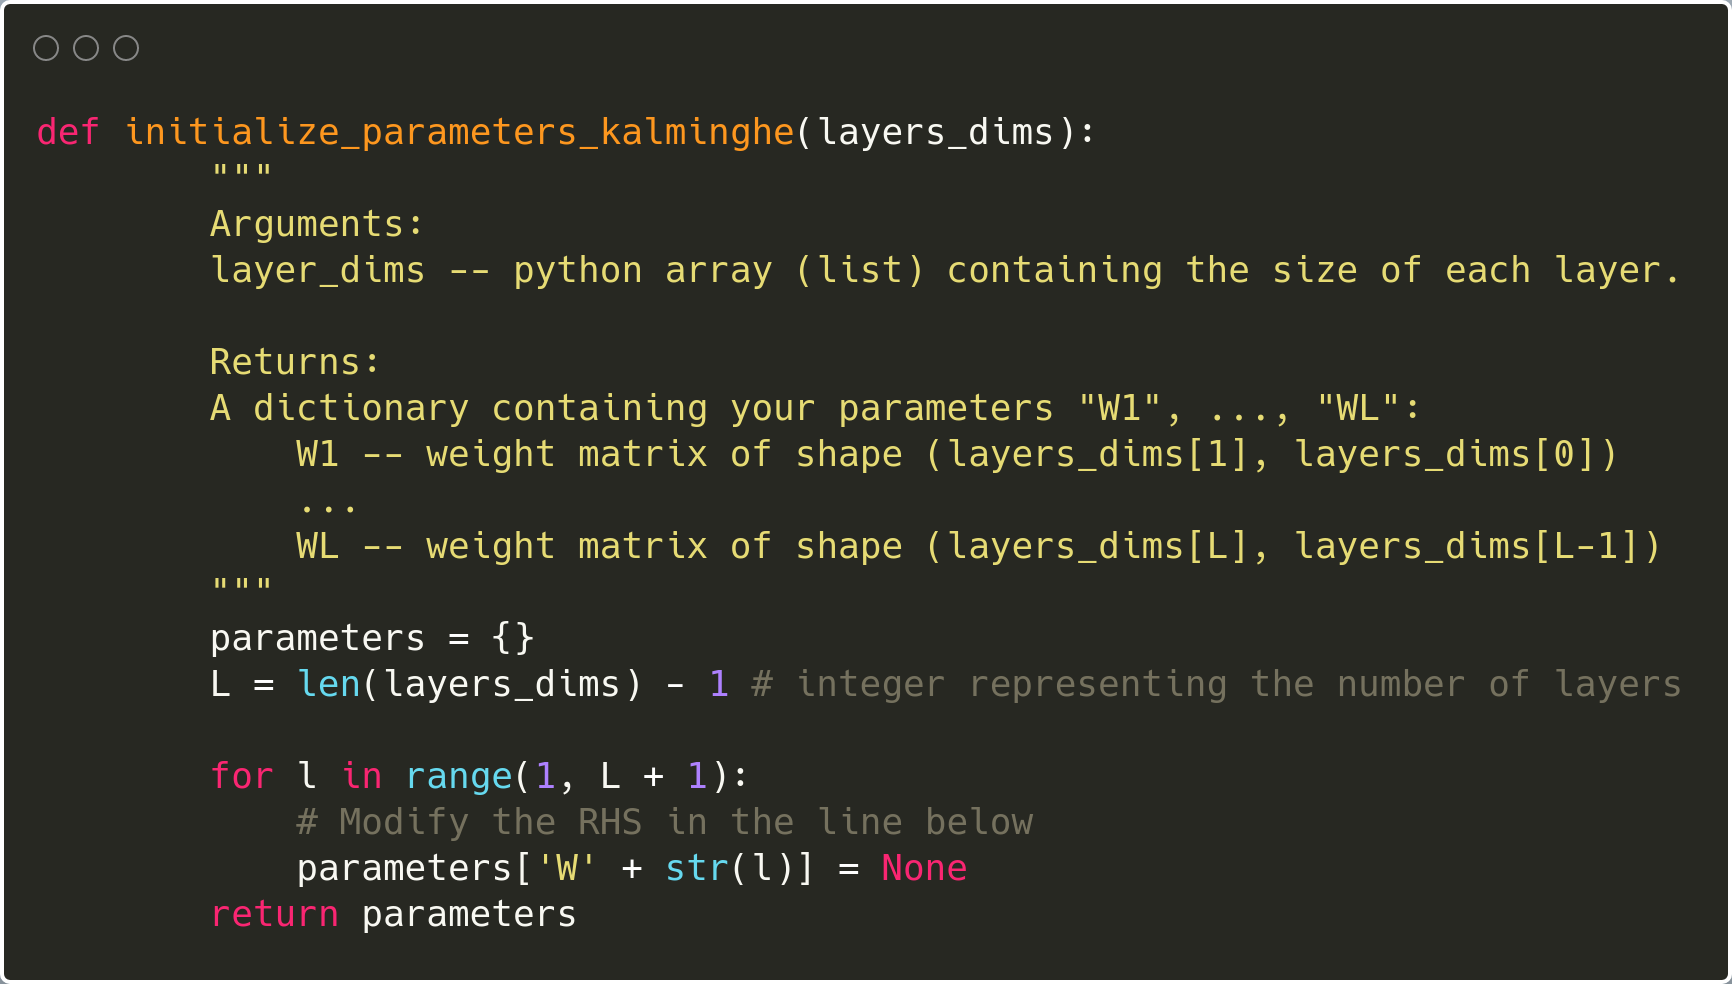
\includegraphics[width=0.8\textwidth]{images/quiz_4_4_1_2.png}

You can use either numpy or PyTorch. Please write the line of code below the comment "Modify the RHS.."


% FIB

\end{frame}
